\documentclass{standalone}
\usepackage{tikz}
\usepackage{nicefrac}
\begin{document}

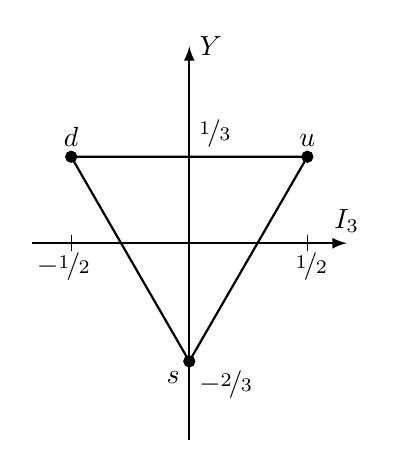
\begin{tikzpicture}

% Definir el tamaño del lado del triángulo equilátero
\def\side{3}

% Coordenadas de los vértices del triángulo equilátero (u, d, s)
\coordinate (d) at (-\side/2, {sqrt(3)/2 * \side});
\coordinate (u) at (\side/2, {sqrt(3)/2 * \side});
\coordinate (s) at (0, 0);


% Dibujar el triángulo equilátero
\draw[thick] (u) -- (d) -- (s) -- cycle;

% Colocar etiquetas para cada partícula
\node[above] at (u) {$u$};
\draw[fill=black] (u) circle (2pt);

\node[above] at (d) {$d$};
\draw[fill=black] (d) circle (2pt);


\node[below left] at (s) {$s$};
\draw[fill=black] (s) circle (2pt);
\node[below right] at (s) {$-\nicefrac{2}{3}$};

%Ejes de la hipercarga e isospin
\draw[-latex, thick] (0,-1)--(0,4) node[right]{$Y$};
\draw[-latex, thick] (-2,1.5)--(2,1.5) node[above]{$I_3$};
\node[below] at(-\side/2-0.1,1.5){$-\nicefrac{1}{2}$};
\draw[fill=black] (-\side/2,1.5-0.1)--(-\side/2,1.5+0.1) ;
\node[below] at(\side/2+0.05,1.5){$\nicefrac{1}{2}$};
\draw[fill=black] (+\side/2,1.5-0.1)--(\side/2,1.5+0.1) ;
\node[above right] at(0,{\side*sqrt(3)/2}) {$\nicefrac{1}{3}$};

\end{tikzpicture}

\end{document}
